\section{Alex Pitcher Report - Part I}

\margininbox{Alex Pitcher, 2011}{As part of the funds coordinated by the Ghar Parau Foundation, on top of £750 towards the general expedition, ICCC received Alex Pitcher memorial fund awards for Jonathon Hardman and Nia John. As Jonathon's report spans the entirety of the expedition, it has been divided into three sections.}{\award}

It had been less than a year since I had embarked on my first trip in a
cave. I had emerged from OFD\sidenote{\passage{Ogof Ffynnon Ddu} cave system in South Wales} thrilled, but following a less enjoyable trip in Yorkshire that had knocked my confidence slightly, I had been apprehensive to accept a place on the trip to Slovenia. After being convinced to come on another caving trip I found myself hooked and it was with a nervous excitement I looked forward to the expedition, unsure of what to expect.

After a week of final preparations -- unfortunately I was absent for most
of them -- we loaded the university minibus full of crates of food and
caving gear and left \passage[town]{London} on the 15\(^{th}\) of July and, departing
across the English channel, I watched the sun set over the white cliffs
of \passage[town]{Dover}: it finally seemed like the expedition had begun.

Unfortunately, not all of the sights to be seen on the drive to Slovenia
were so romantic. The van sped through Belgium and Luxembourg before the
monotonous Autobahn provided an apt lesson in `how to fall asleep in
uncomfortable positions.' Despite the long journey time (roughly 24
hours), it didn't seem like all that long before we arrived in Slovenia
where the scenery took a turn for the more dramatic. Upon crossing the
border we were at once surrounded by dramatic mountains cut through by
rivers of striking turquoise: our home for the next month.

Arriving in \passage[town]{Tolmin} -- the local town and `base of operations' if you will --
we were greeted by three more members of the expedition and a sweet can
of Laško, the local beer, at the flat of James ``Tetley'' Hooper.
Already dark we headed to the local pizzeria, an ICCC staple in
Slovenia, and listened to the older members of the group exchange
stories of various caving trips that had taken place within the
mountain. I listened intently, filled with excitement and trepidation
knowing that soon, I could be seeing the \bignote{vast cavernous pitches that
apparently dwarfed anything I had seen in the UK, the thoughts of which
ensured I had a restless sleep that night}.

The first task that was to be faced was the setting up of a camp on top
of the mountain. The supplies that we had stocked the van up with before
leaving \passage[town]{London} had to be carried up the mountain for use and the only
viable way of doing this was by loading up our rucksacks and carrying
the loads up ourselves. To make this a little easier, we drove an hour
outside of \passage[town]{Tolmin} up some precarious mountain roads -- special mention to
the drivers who did an excellent job -- to the small village of \passage[town]{Tolminske
Ravne}.

\tweet{11:16AM Jul 17, 2011}{6AM start to get the carries in,no helicopters on this expo!Weather kind, overcast,cool but dry.All 11 up top tonight, peaceful on Migovec.}

Here we were greeted by the family who had set up a deal with the
expedition to allow us to use their barn to store our supplies in. The
family were, like almost every Slovenian I met, very welcoming and
greeted us with a strong coffee to waken us up for the carries and a
shot of Jagenje, a spirit fermented from pears. With my body now trying
to figure out what the hell I had just drunk we unloaded the van and,
for the first time loaded our rucksacks under the shadow of \passage[mountain]{Migovec} for
the first carry.


	\begin{figure*}[t!]
	\checkoddpage \ifoddpage \forcerectofloat \else \forceversofloat \fi
		\centering
  		\begin{subfigure}{\textwidth}
			\centering
			\frame{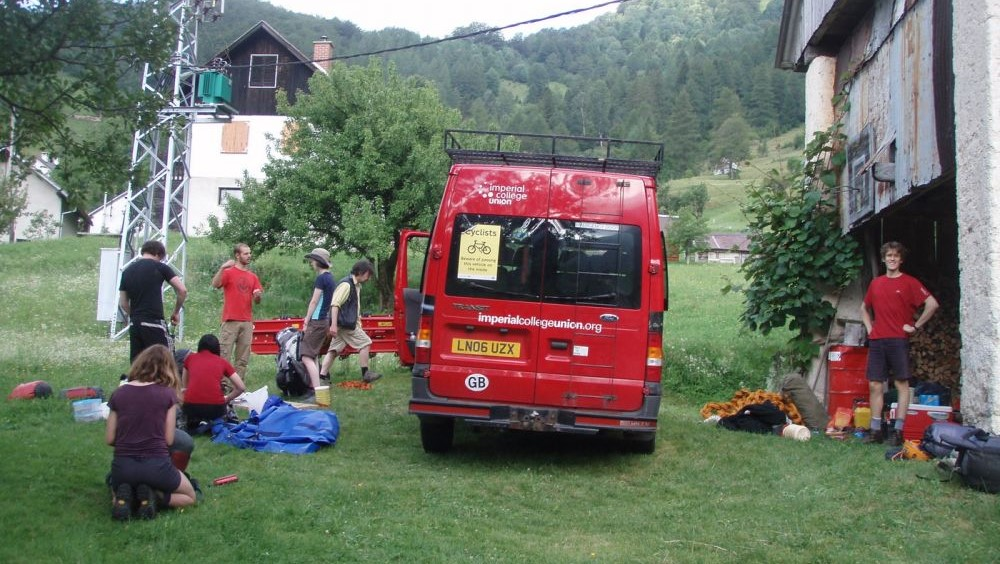
\includegraphics[width=\linewidth]{2011/alex_pitcher_award/2011-07-17-07.57.23-Jan Evetts-Olympus Compact-P7170001-Arrival at Ravne--orig_1050p.jpg}}
			\caption{}
			\label{ravne arrival 2011}
		\end{subfigure}
    \vspace{0cm}
		\begin{subfigure}[t]{0.49\textwidth}
			\centering
			\frame{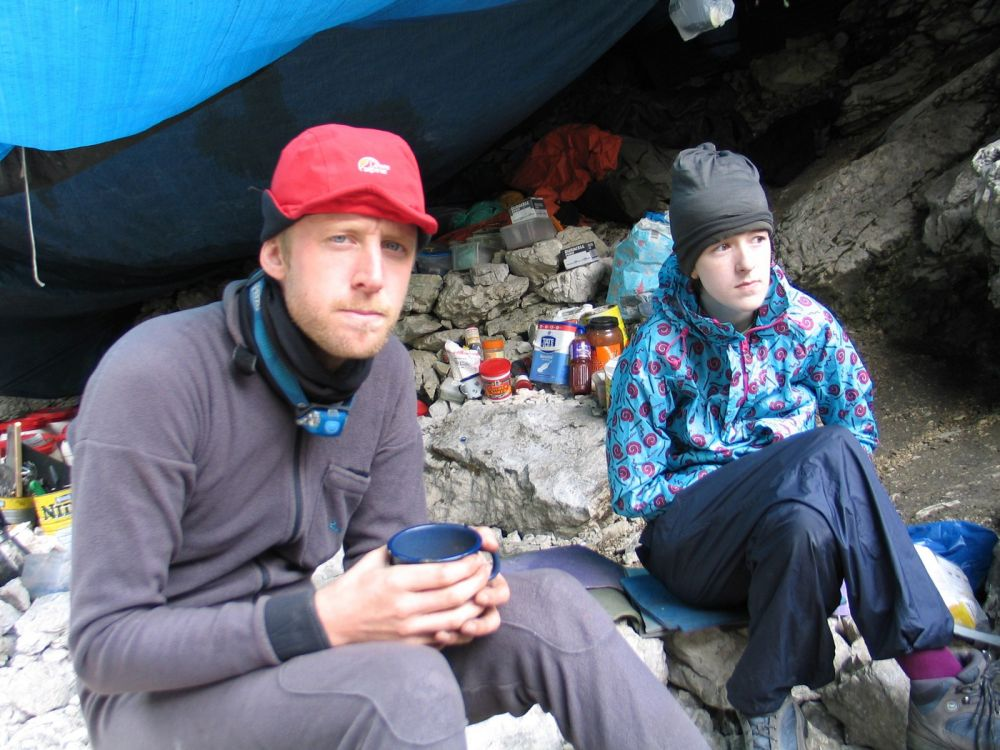
\includegraphics[width=\linewidth]{2011/alex_pitcher_award/2011-07-20-13.52.27-Jarvist Frost-CanonG5-IMG_0112 - Jan and Nia in the Bivi--orig_1050p.jpg}}
			\caption{}
			\label{jan nia}
		\end{subfigure}
	\hfill
		\begin{subfigure}[t]{0.49\textwidth}
			\centering
			\frame{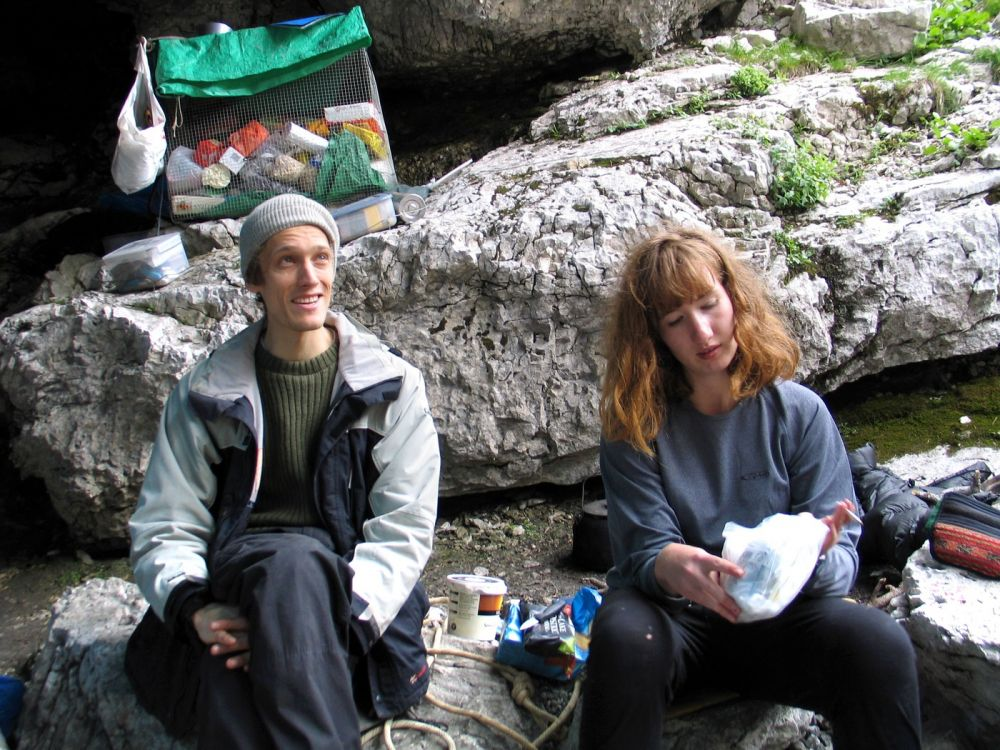
\includegraphics[width=\linewidth]{2011/alex_pitcher_award/2011-07-20-13.52.44-Jarvist Frost-CanonG5-IMG_0114 - Jarv and Kate in the Bivi--orig_1050p.jpg}}
			\caption{}\label{jarv kate}
		\end{subfigure}
		\caption{Settling in.
  \textit{(a)} The minibus at \passage[town]{Ravne}, parked outside the Skalar family's barn. \pic{Jan Evetts.}
  \textit{(b)} Jan and Nia John in the bivi, alongside 
  \textit{(c)} Jarv and Kate. \pic{Jarvist Frost.}}
	\end{figure*}


The carries up took roughly three hours to (by the end of the expedition)
two hours for myself and, as perverted as it may seem, I really enjoyed
them. The first half of the carries were, to be honest, fairly
uninspiring as the path ascended quite steeply through a forest towards
the tree line. On hot days, this section seemed to drag on but once a
few carries were out of the way and all the shortcuts learnt it was
possible to briskly trudge through the steeper sections and enjoy the
more level sections and the breaks they provided. Upon exiting the
tree-line the passing hiker is greeted by three shepherd huts. This made
a sensible halfway home from \passage[town]{Ravne} and was also a welcome drinks
break. The next section of the hike was much more spectacular and
enjoyable. A group of zig-zagging bends lead up to a path that then
curves round the side of the mountain, negotiating a couple of quite
tiring scree-slopes. Below the raw a river can be heard as it descends
into the Tolmin valley whilst the mountain \passage[mountain]{Krn} -- the site of a front in
WW1 -- rears imposingly out of the other side of the valley. After
negotiating round the back of \passage[mountain]{Migovec} the portal was eventually reached.
Quite simply, this was the point that, upon crossing, lead into the
\passage{Migovec Plateau}: the site of our camp.

\tweet{9:19PM Jul 17, 2011}{Rain\& klag attack for 2nd half of play,carries continued regardless.First meal up top-risotto.UG camp carry tom AM,talk of adv rig team PM! }

Stepping through the portal for the first time I was excited to finally
see the Bivouac where we would set up camp, a site I had repeatedly read
about in previous expeditions before joining the expedition. I would say
that it immediately felt like home but, really, when I arrived it was
just a fairly unassuming rock bridge that was yet to be set up as camp.
After having a break and enlisting some help to setup the tent I would
be sleeping in, I was given a guided tour of the plateau and then I headed down
the mountain to embark on a second carry.


\fullwidthbox[\logbook]{The card game \textbf{Presidents And Arseholes}, an old staple}{

\textbf{Objective}

Get rid of your cards.

\textbf{Ranks}

Suits don't matter. Aces high. Use two decks if people>7. Doesn't matter if people start with different numbers of cards.

\textbf{Rules}

First person starts with i.e. two 7s. Following person has to either pass, or play a higher set i.e. two Jacks. After a full round of passing, played cards are turned over and person to left starts play again. Do not have to play, can pass then play etc.

\textbf{P\&A}

First person to get rid of cards is President, second is Vice President. Last two are Vice Arsehole and Arsehole.

On next round, Arsehole gives two highest ranking cards to Pres, Pres gives two worst (his choice) to arsehole. Same for vice pres + vice arse, except one card.

\textbf{Cheating}

Strongly encouraged. In particular, hiding other cards below the correct top card (i.e. putting down 3,4,5,5 instead of 5,5,5,5) works quite well.
}


Returning to the Bivi, it felt more like home with more people occupying
it and with many more supplies laying strewn across its floor. Already,
however, it had begun to rain quite heavily on the plateau. The
expedition sat for a while, as we ate our fondly named `slop' (although
it was anything but; we ate very well most of the time on the plateau)
and exchanged stories and plans whilst warming ourselves up with
whiskey. It wasn't long before I retired to the comfort of the tent I
was staying in, nicknamed the Casino for its large size that can
accommodate card games.


\begin{marginfigure}
\checkoddpage \ifoddpage \forcerectofloat \else \forceversofloat \fi
\centering
 \frame{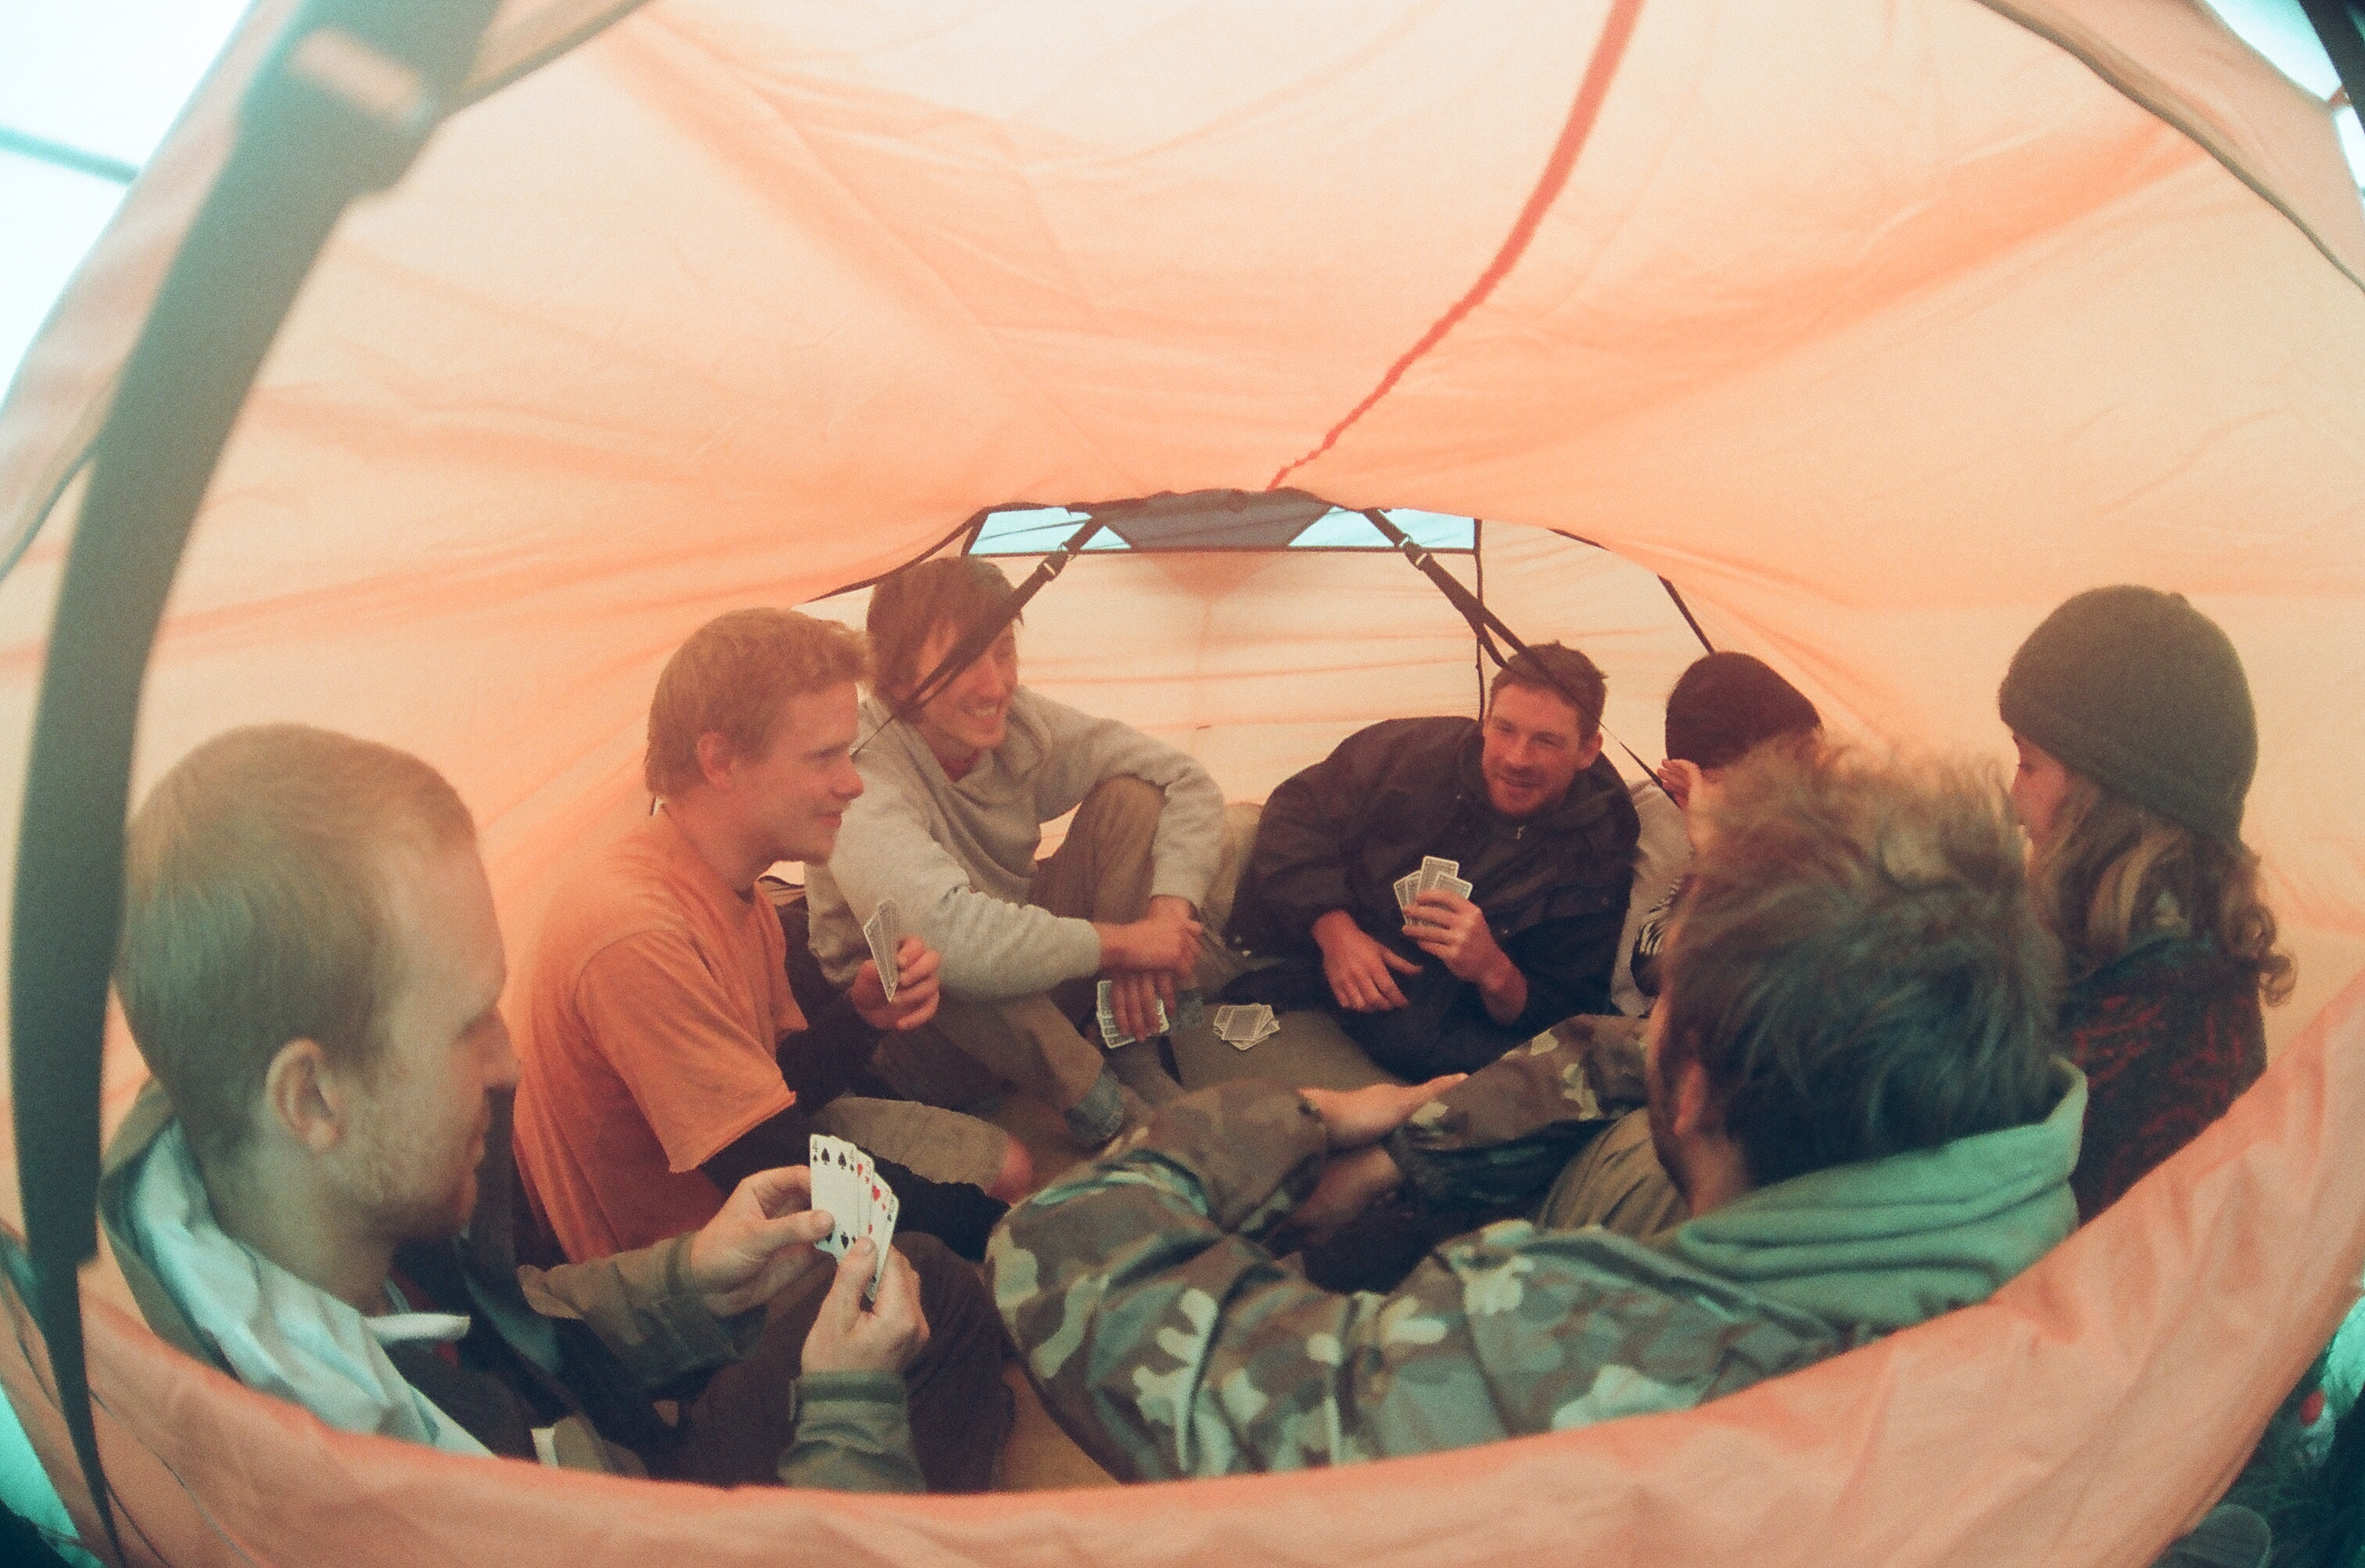
\includegraphics[width=\linewidth]{2011/alex_pitcher_award/Jarvist Frost - Canon A1 Zenit 16mm - 61320033--orig.jpg}} 
 \caption{The Casino, as the largest tent, is a frequent sanctuary for those who haven't yet drifted down to the bivi. \pic{Jarvist Frost}}
 \label{playing cards}
\end{marginfigure}


Upon finding sleep I was awakened at around 1
o'clock in the morning by the sound of thunder and heavy rain pounding
the side of our tent. Feeling quite exposed being so high up on the
mountain I lay still, wide-awake, listening to the thunder move closer
and closer to our position. It wasn't too long before I heard the zip of
our tent fly open as Kate -- another fellow undergraduate -- flew into the
Casino. Having been convinced to pitch her tent on a stretch of ground
that she would later find out was called lightening ridge she was
understandably nervous and so, came to ours for some comfort. It also
became apparent that we had all been awake and, after some joking about
the storm, I settled down and fell into a deep sleep.

Over the next few days we continued with the carries yet morale seemed to
be rather low after the storm and the soaking of people's equipment and
tents that came with it (I learnt quickly it's never a smart idea to
leave books in the porch of the tent overnight). Slowly and sombrely,
the more experienced cavers began to move underground and rig the cave.
It was prior to the rigging of camp that one of the older cavers offered
to take me underground in Slovenia for the first time.

	\begin{figure*}[t!]
	\checkoddpage \ifoddpage \forcerectofloat \else \forceversofloat \fi
		\centering
		\begin{subfigure}[t]{0.49\textwidth}
			\centering
			\frame{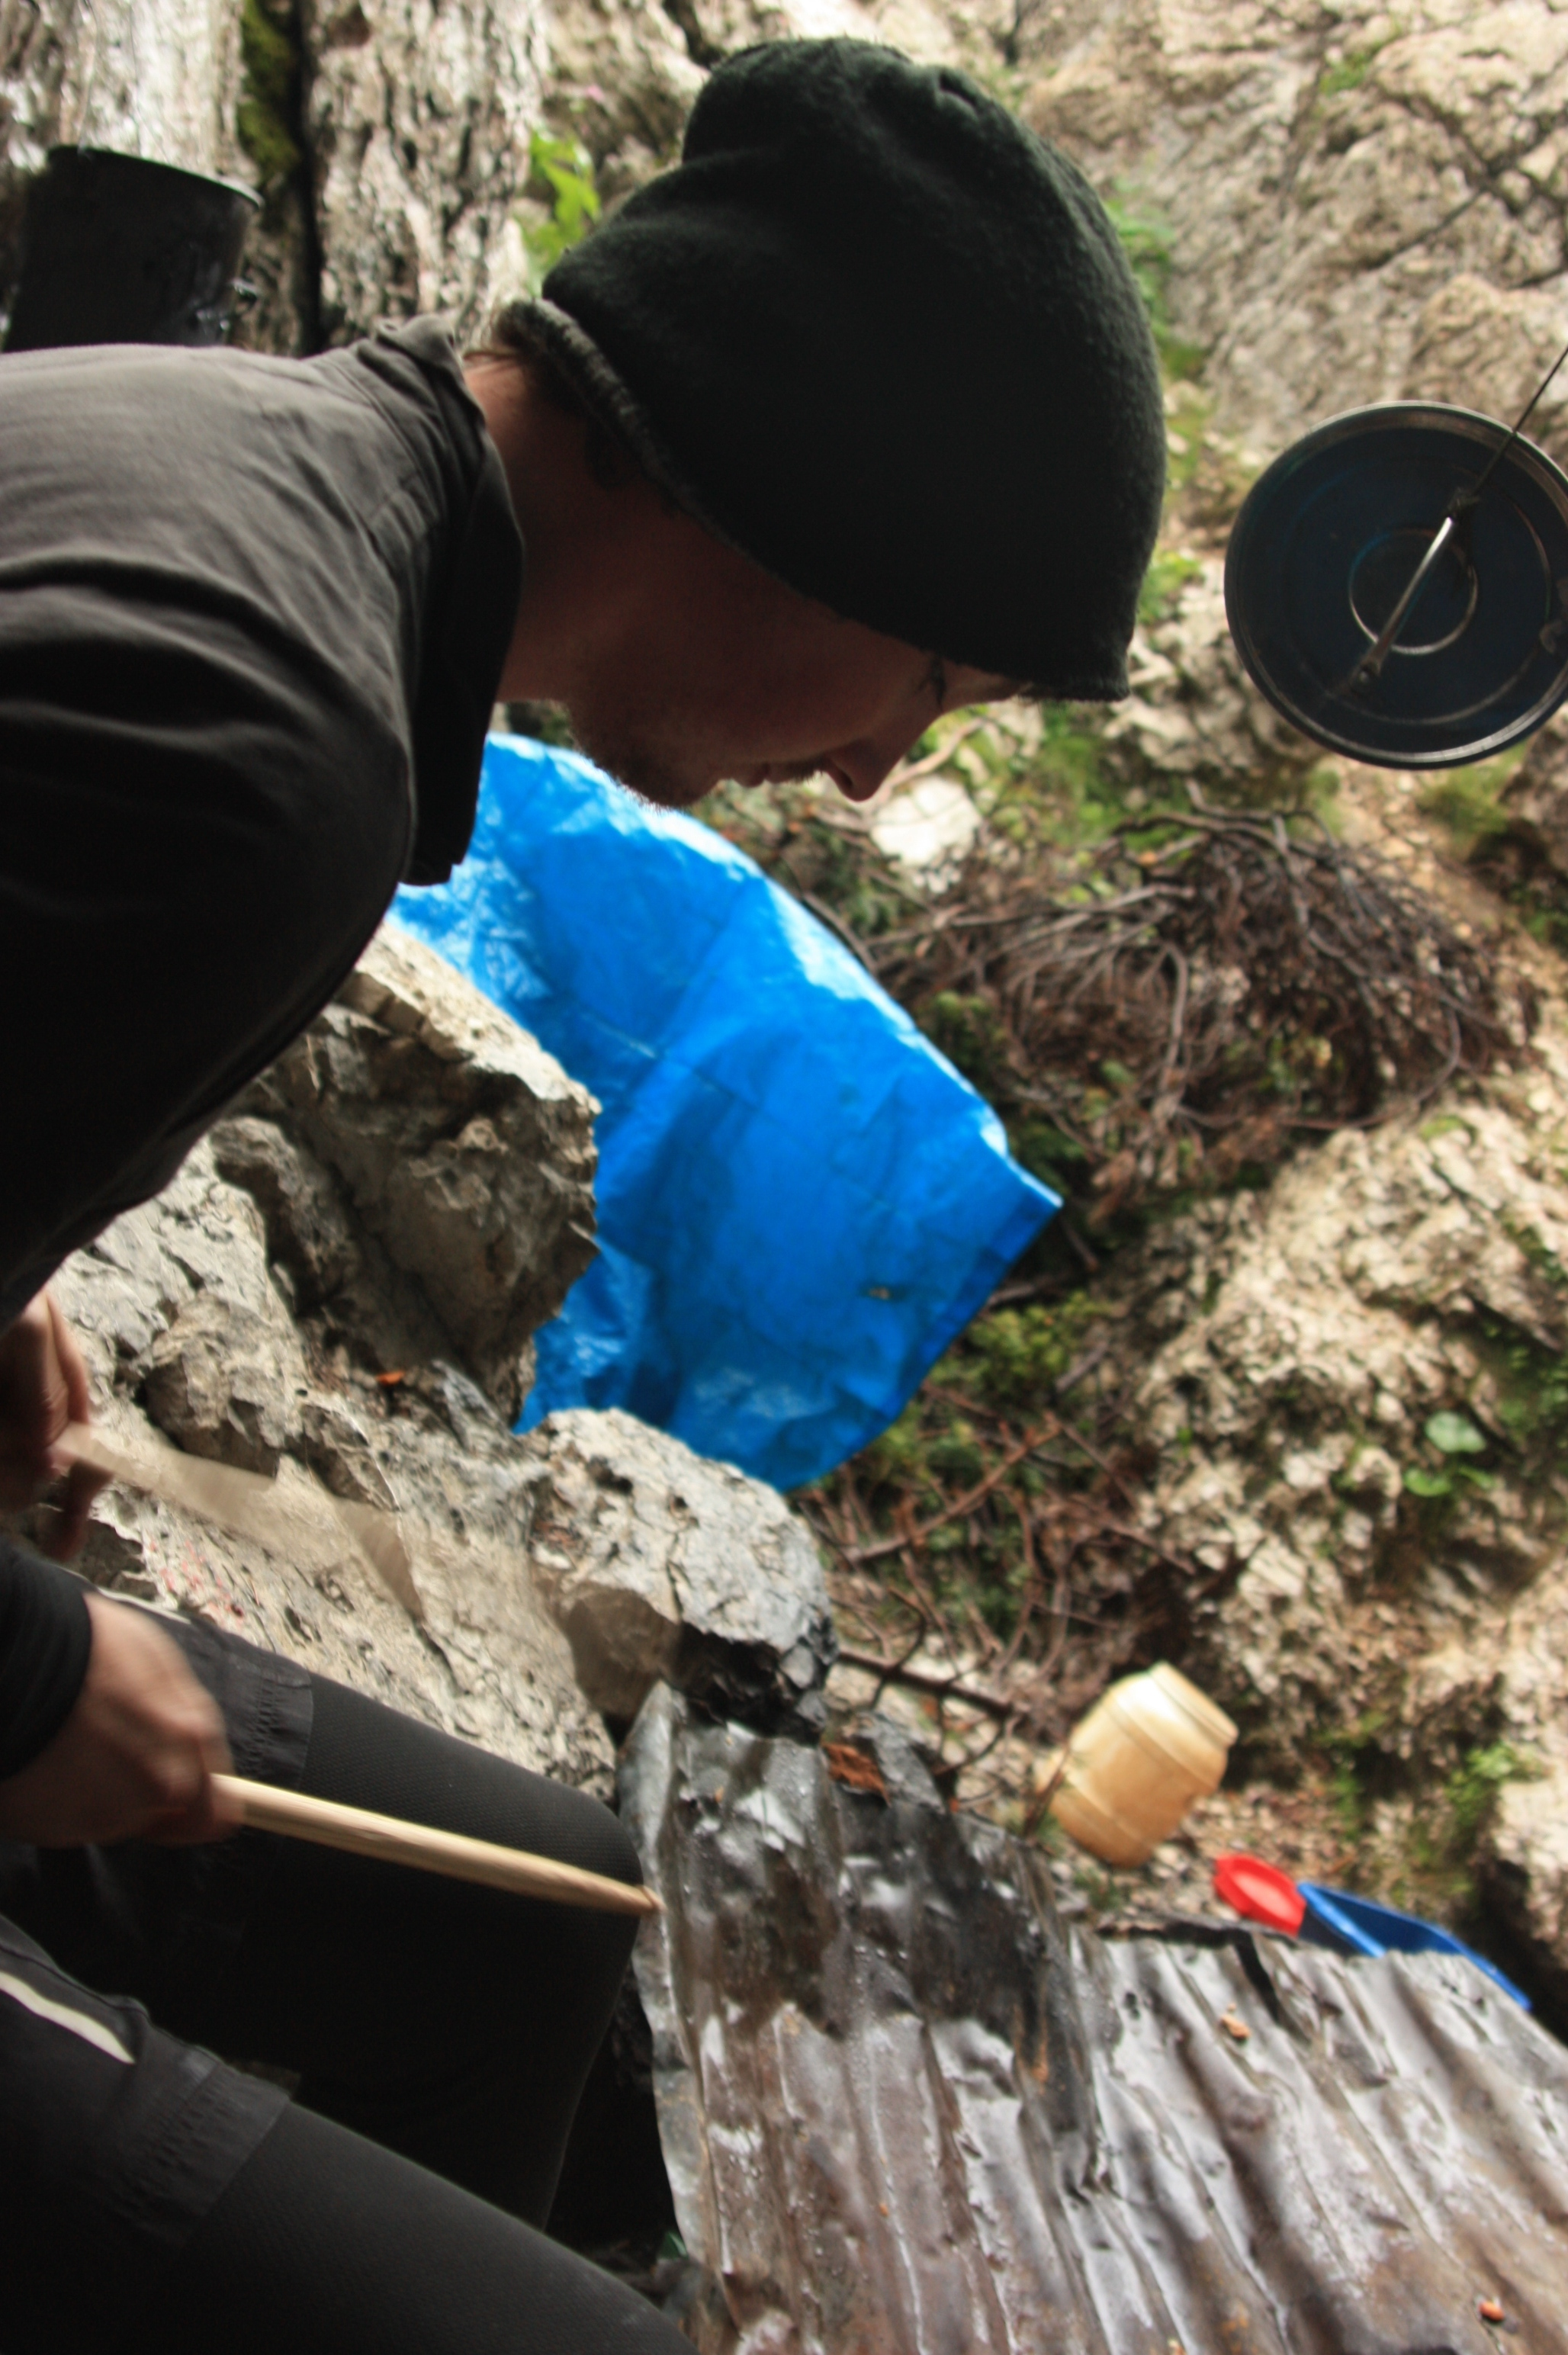
\includegraphics[width=\linewidth]{2011/alex_pitcher_award/2011-08-06-13.42.26-Gergely Ambrus-Canon450D-IMG_1013-Wet Cold Bivi--orig.jpg}}
			\caption{}
			\label{Bivi drums}
		\end{subfigure}
	\hfill
		\begin{subfigure}[t]{0.49\textwidth}
			\centering
			\frame{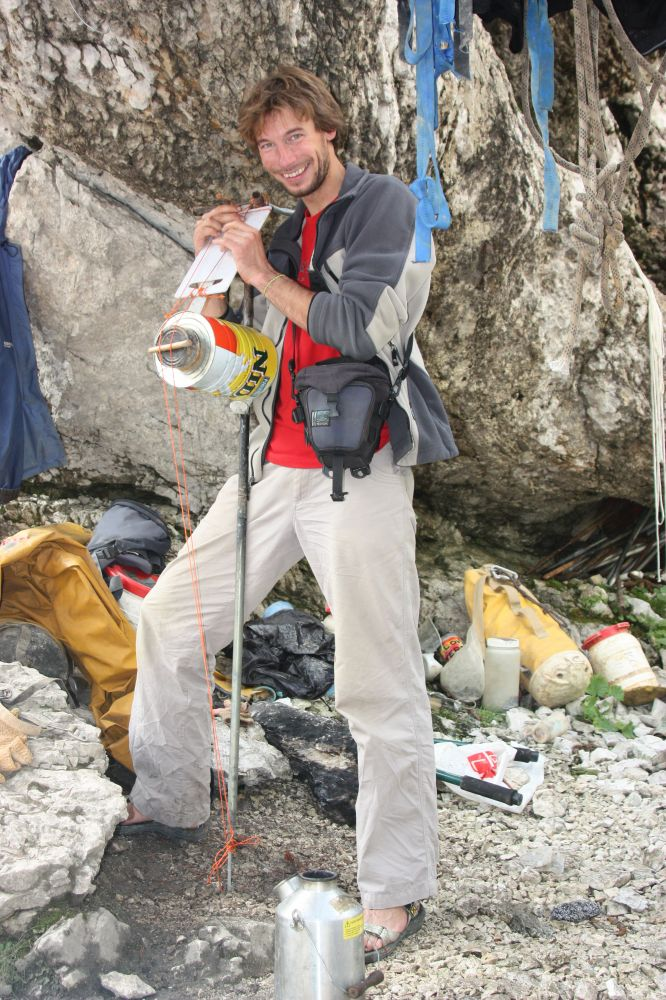
\includegraphics[width=\linewidth]{2011/alex_pitcher_award/2011-08-10-09.41.19-Gergely Ambrus-Canon450D-IMG_1248-Bivi Stringed Instrument--orig.jpg}}
			\caption{}\label{Bivi Stringed Instrument}
		\end{subfigure}
		\caption{A regular expo occurrence is the construction of musical instruments from bivi items (old Nido tins, tent poles, etc). Every bivi instrument is unique.
  \textit{(a)} Jonny playing a makeshift drumkit, including among its components a well-hung saucepan and the metal sheet normally used as a fireguard.
  \textit{(b)} The "stringed instrument" of 2011. \pic{Gergely Ambrus.}}
	\end{figure*}



\subsection{First trip underground}

The caver in question was Tetley, somebody I had been caving with once
before in the \passage{Mendips}. The cave in question was \passage{Swildon's Hole} and, as
such, he had no idea if I was any good at SRT and had to place a lot of
faith in me not to do anything stupid. I, on the other hand, had a lot
of trust in him, knowing that he had a lot of caving experience, having
been on the expedition for around 10 years, prior to that attending the
Oxford expeditions in the \passage{Picos}. He did, however, seem slightly mad but
that only added to the sense of adventure.

The cave that we were to be surveying this year had once been known as
`Ben's Crap Lead' but was renamed to `\passage{Vrtnarija}' (meaning
Gardener's World) when the cave went big upon the discovery of a 60 m
pitch named \passage{Pico}. Since the initial years of discovery the cave had now
reached a length of 8776 m and a depth of 877 m and had presented a
number of exciting potential leads for the expedition. My trip was a
much more pedestrian affair that was to take me to the top of a pitch
named \passage{Tessellator}, just over 200 m down. To me this was no
laughing matter. Prior to Slovenia I had acquired limited SRT experience
to put it lightly. The three trips I had been on that contained SRT,
moreover, had also not been very deep. Finally, I hadn't necessarily
performed very well and wasn't very confident. In the grand scheme of
things, the trip was merely a brief peak into the entrance series of the
cave; for me \bignote{it was already deeper than I had ever been} containing more
re-belays and deviations than I had seen throughout the whole year in
the UK.

Descending down the first few pitches, I felt fairly rusty as I bumbled
through the cave yet, despite this, I felt at ease with my SRT, certain
that I could make it up and down the rope safely, if not efficiently.
Descending through the entrance series, I had the opportunity to make a
mess of my first attempt at putting a bolt in which gave me my first
glimpse at the patience needed for expedition caving (even if it was
only one bolt). Otherwise, the cave was fairly unassuming until I
arrived at the first large(ish) pitch named \passage{Laurel}. Descending first,
Tetley told me to watch out for an annoying deviation and descended down
the pitch. Soon after \bignote{I heard him call out from the dark, ``JOONNYY!!
I'VE GOT THE FEEAARR!'' followed by his unmistakable giggle}. Wondering
what was down there I descended down the pitch passing the deviation
with a small amount of annoyance and reached the re-belay he was talking
about. Walking out onto a rock bridge below me there was a large drop
leading to a ledge about 30 m down. Heading to the edge of the rock ledge,
safely secured by my cowstails, I clipped onto the rope with my
descender, knees shaking, and descended down to the ledge. I must have
arrived at the bottom beaming. Despite the descent becoming `just
another pitch' by the end of the expedition it had given me my first
taste of the large drops and exposure that made Slovenia so different
from the UK -- I was hooked.

The next set of pitches was known as the \passage{Urinal Series}, much smaller in
scale yet much more annoying due to their awkward pitch heads. Not being
the most graceful of cave-goers I went for \bignote{the questionable technique of
pushing my way through the tighter pitches} despite being warned about
the sharp rock that is to be found in caves not worn down by generations
of cavers (this would later come back to haunt me in the form of a torn
oversuit).

Following the \passage{Urinal Series} I arrived at my first big pitch. Before me
the cave opened up into a seemingly bottomless hole. Tetley asked if I
wanted to go any further and, excited at the thought of going further
into the cave I eagerly agreed. The pitch itself was really quite nice
the first time down. It was a nice amble down six re-belays -- good
practice for my SRT. At the bottom we decided to head down a few more
pitches to the top of a pitch named \passage{Tessellator}, the pitch head of
which was supposedly quite tight and, not being a small guy, had me
slightly nervous. Arriving at the top of the pitch I realised I had
nothing to worry about and, as it had taken me awhile to get this far,
we decided to turn back, especially as it was my first trip.


\begin{marginfigure}
\checkoddpage \ifoddpage \forcerectofloat \else \forceversofloat \fi
\centering
 \frame{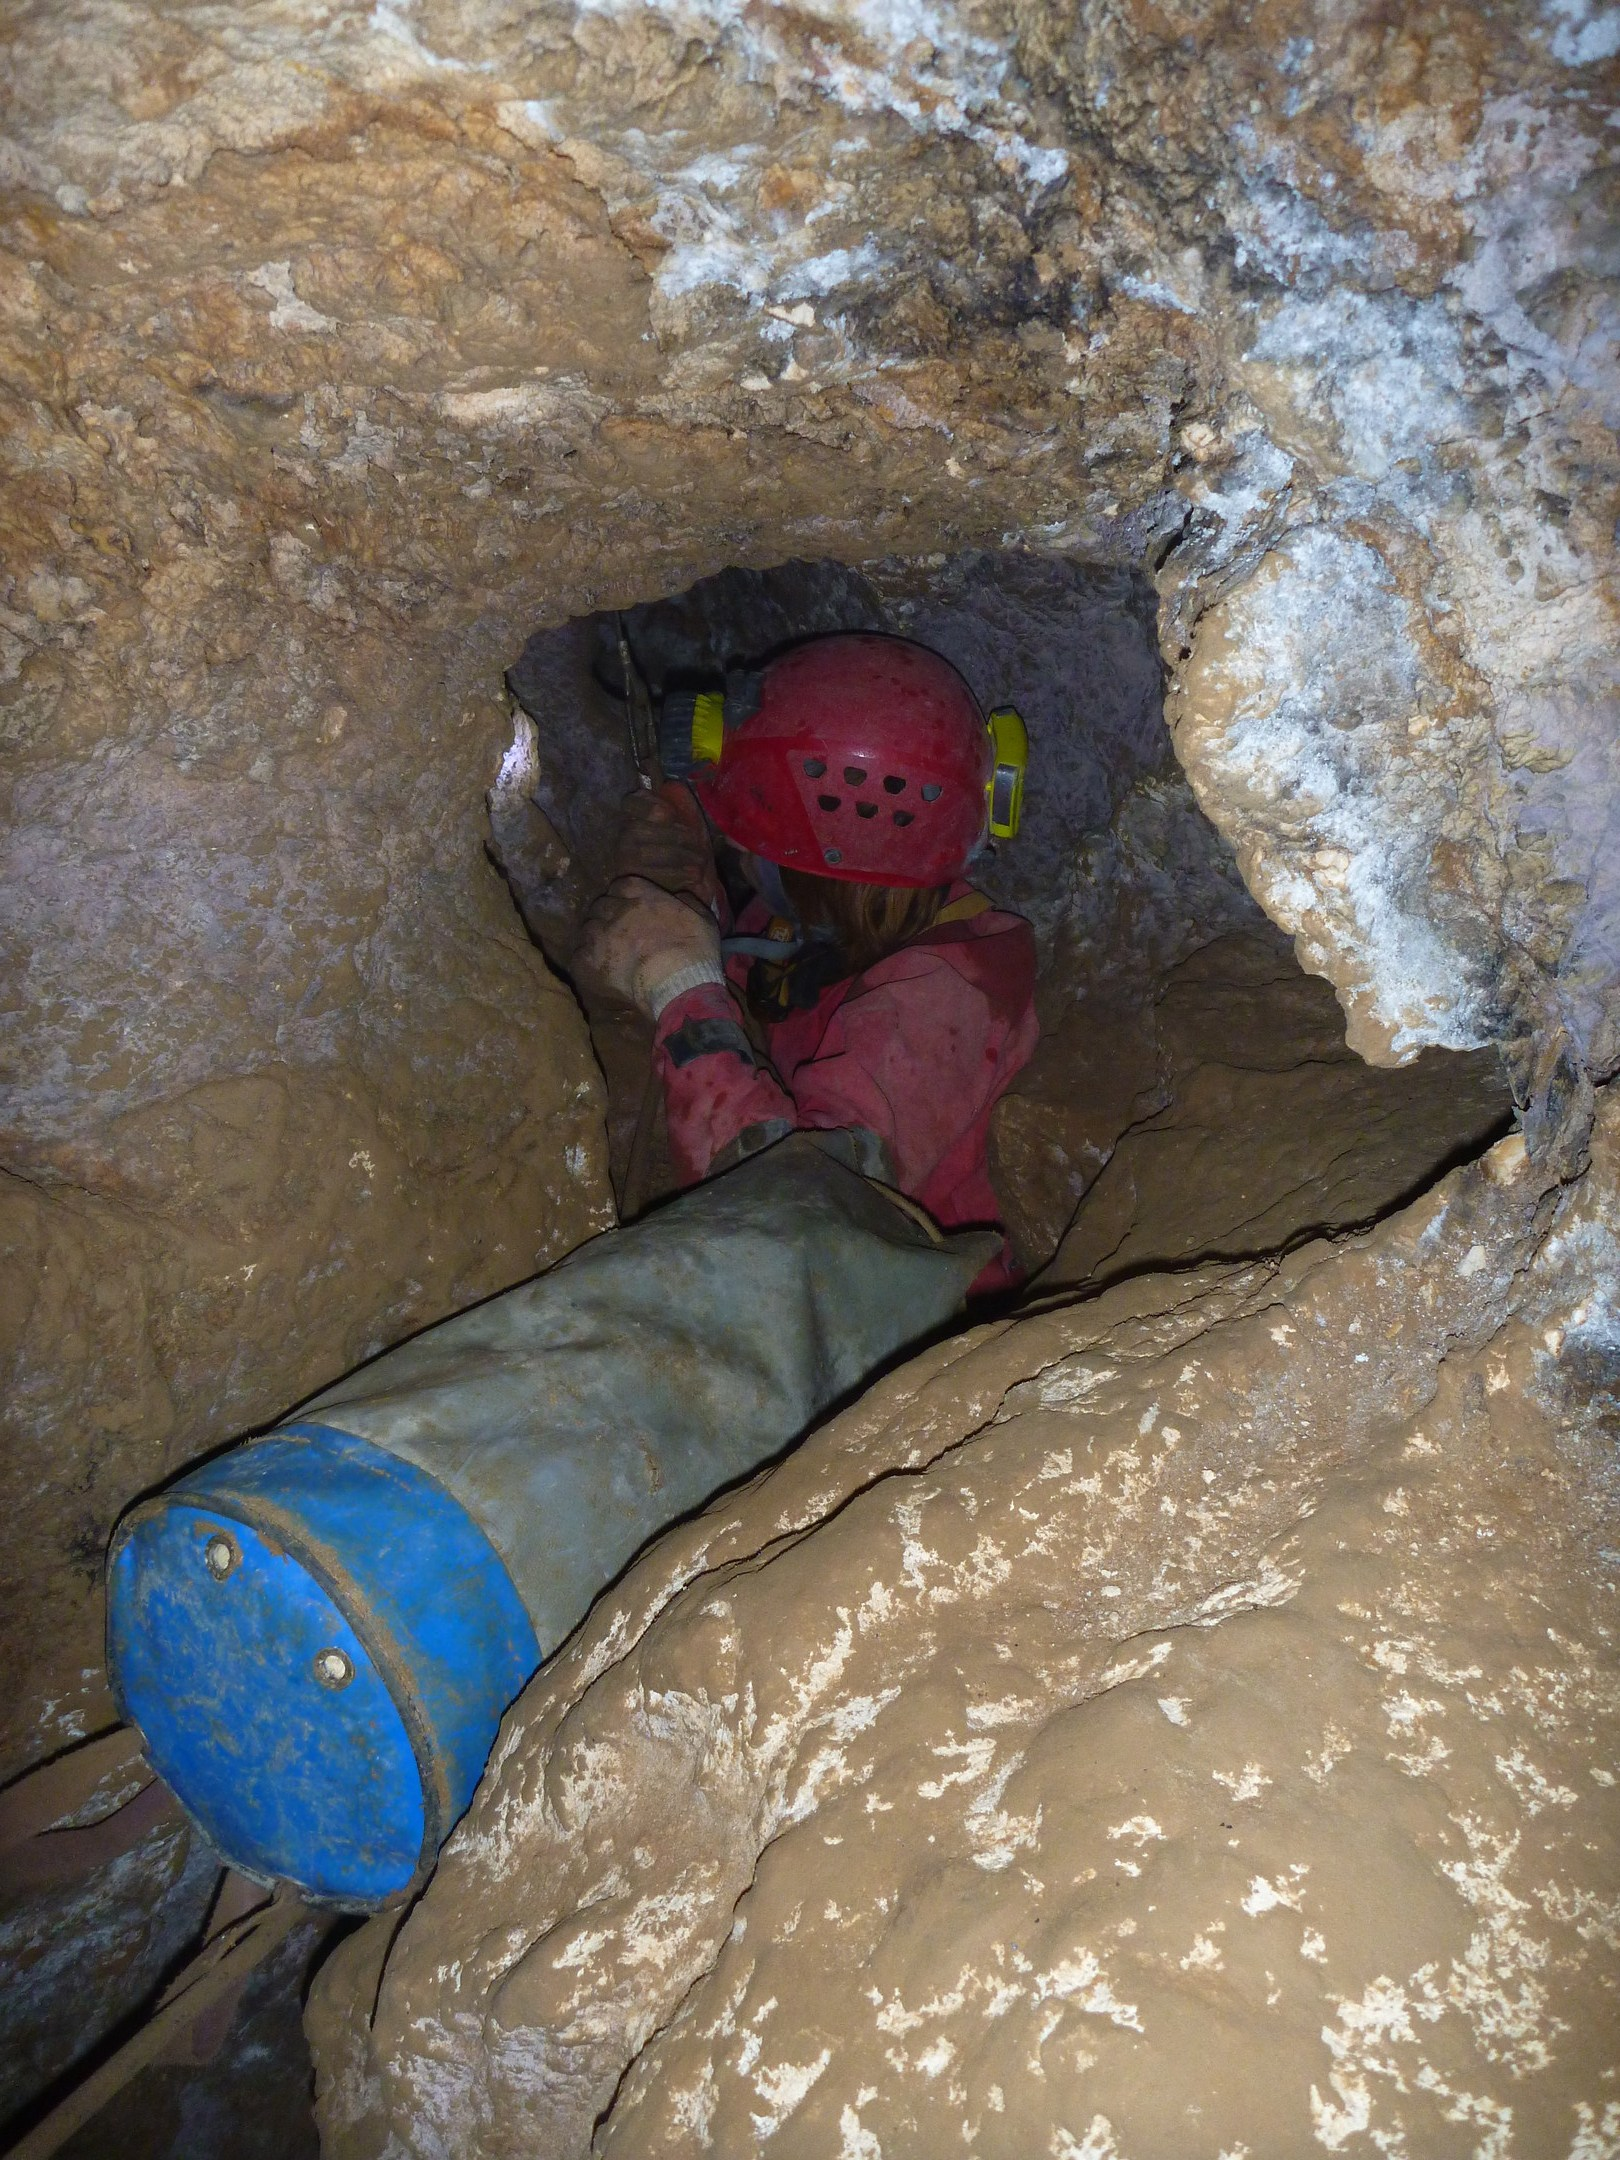
\includegraphics[width=\linewidth]{2011/alex_pitcher_award/2011-08-01-13.30.55-Grega-Panasonc DMC-FT2-079-tesselator pitch head--orig.jpg}} 
 \caption{Tjaša Rutar passing the \passage{Tessellator} pitch head. \pic{Grega Maffi}}
 \label{tjasa tessellator pitch head}
\end{marginfigure}


The journey out was more of a challenge. At this point, whilst my SRT
was getting better, my prussiking hadn't been assessed yet and, frankly,
it was fairly awful. Moving slowly up through \passage{Pico} and awkwardly making
my way out of the \passage{Urinal Series} we met up with another group of cavers
on their way down to set up camp. It's generally always enjoyable to
meet other cavers in a cave and this was probably an exception for the
others as Tetley had early changed an awkward deviation into an awkward
re-belay much to their contempt. They passed by quite grumpily much to
our amusement, a feeling that may have been heightened by the miserable
weather we had had on the surface. Arriving at the entrance of the cave
after roughly 4 hours I was quite tired yet I felt much more confident
in my SRT, even if I was yet to learn how to be efficient.

On the surface, a can of beer was exchanged and we made a plan to go to
camp in the next couple of days. I spent the next day lazing around
reading and partaking in another carry up the hill. The day after, we
set up our gear and descended into the cave for my first trip to camp.

\subsection{First trip to underground camp and pushing}

Already I felt much more at ease with the cave as I made much quicker
progress to the bottom of \passage{Pico} than I had done on the previous trip. In
what felt like no time at all I arrived at the top of \passage{Tessellator}
and slipped through the narrow pitch-head with no trouble at all.
Suddenly, my nerves became more apparent at the thought of descending
deeper into the cave. Almost all the pitches from now on were roughly
the same height as \passage{Pico}, if not larger and in no time at all, I felt
myself committing myself to a much greater depth to ascend from. Despite
my nerves, I knew that I would be able to get out from where I was and
we continued deeper and deeper down, as the maximum depth I had found
myself in a cave ratcheted up as did the number of pitches:
\passage{Tessellator}, \passage{Space Odyssey}, \passage{Concorde}, \passage{Alchemy},
\passage{Fistful of Tolars}.

\margininbox{22-07-2011 7:45 pm}{

Johnny and Tetley arrived at \passage{X-Ray} after a smooth 4hr journey
down. It's good to be back! Fairy lights\ldots{} not so sure about
them\ldots{} Cup of tea then off for a tourist trip down \passage{Friendship Gallery}. \name{Tetley}}{\logbook}

Now, vertically I was very close to camp, I just had
to pass through an awkward section of cave that followed an old fault
line known as \passage{Pink} and descend a couple of pitches. Despite being
told that I may find \passage{Pink} slightly awkward (I'm quite a broad
person) I found it no problem going down compared to some of the tight
sections I had experienced in the UK as was the case with most of
Slovenia. Finally I was at the bottom of \passage{Zimmer}, the final pitch
before camp staring up at the seemingly never-ending blackness above me.
Arriving at camp, we decided to undertake a tour of the horizontal
section of cave we were in known as \passage{Friendship Gallery}. Here, the
caving was much more like the phreatic sections of cave I had
experienced in \passage{Swildon's Hole}. It led to one of the largest pitches in
\passage{Gardener's World}, the wonderfully named \passage{Big Rock Candy Mountain}.
The entrance, however, was pretty unspectacular: just a man sized hole
leading to a mud slope. Following this we decided to return to camp
where a meal of fishy soupy cheesy smash and a long sleep waited.

\margininbox{22.07 - what time\ldots{}}{

Camp appears to be comfier than bivi! Looking forward to starting pushing tomorrow. \name{Jonny Hardman}}{\logbook}


\begin{pagefigure}
\checkoddpage \ifoddpage \forcerectofloat \else \forceversofloat \fi
   \centering
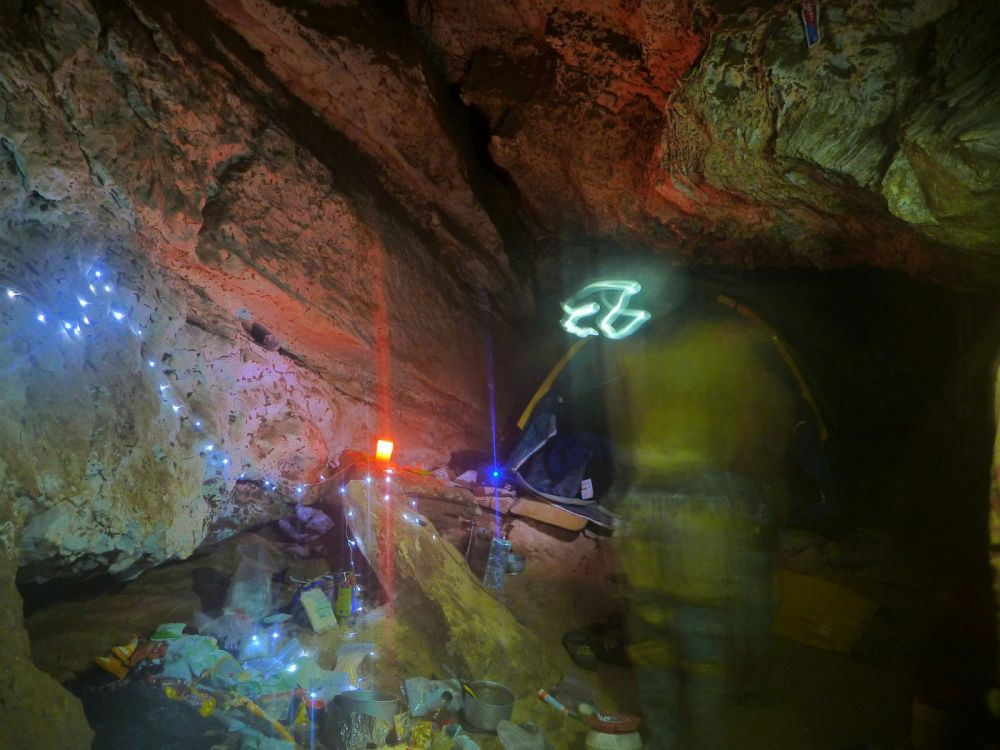
\includegraphics[width = \textwidth]{2011/alex_pitcher_award/2011-08-03-10.32.46-Grega-Panasonc DMC-FT2-106-camp x-ray--orig_1050p.jpg}
\caption{Fairy lights (left) were a new -- and ultimately welcome -- addition to camp \passage{X-Ray} in 2011. Powered by ordinary AA batteries, they add comfort as well as extra lighting to the camp. \pic{Grega Maffi}} \label{fairy lights camp}
\end{pagefigure}



The following day we woke up and got ready slowly to go to look at a
lead that had been found the previous year. The weight of the surface
was beginning to weigh on me but I was excited to see if we could
discover some new cave. Heading back to \passage{Zimmer} we descended down
a pitch named \passage{Cheetah}, a wonderful pitch with a welcoming mud
slope at the beginning. Following instructions left from last year we
made our way through some passages known as the \passage{Wonderland} series
before arriving at what seem liked a ledge of boulders halfway down a
pitch. Quite remarkably, a caver known as Dave had found a lead
underneath this pile of boulders last year whilst waiting for another
caver to rig a pitch. We were to explore this section of the cave.
First, however, I had to get through my first truly awkward piece of
cave in Slovenia. To get through to the section of cave he had found,
Dave had descended through a narrow hole that to others may have been a
fairly easy squeeze. To me, however, it was impassable and, \bignote{arming
myself with a hammer I began to chip away at the hole} whilst Tetley had
a look at the lead. Further down the passage he seemed excited at the
prospect of a horizontal lead and returned to chip in with the
hammering. It didn't take too long before I was through and walking into
uncharted cave.

\margininbox{Red Baron}{
     \begin{itemize}
    \item Jonathon Hardman
    \item James "Tetley" Hooper
    \end{itemize}}{\explo}

Rather unassuming to begin with, a section of cave with low roof seemed
to following a bedding place before opening up into a fairly expansive
chamber. At the end of it was a 10 m hole in the ground, on the other
side of which there was what seemed to be another horizontal section of
cave. I was ecstatic and \bignote{couldn't quite get my head round being the
first two people ever to step on this piece of the earth}. We returned
back to the beginning and surveyed the section of cave, naming it the \passage{Red Baron} after the Blackadder episode we had watched the night
before.

Before considering the traverse to the other side of the hole we decided
to have a look at the lead that had been found the year before,
\passage{Kamikaze}, and to see if it continued. \passage{Kamikaze} turned out
to be an uncomfortable stretch of cave. It quickly degenerated from a
crouch to a crawl up a bedding plane that was anything but enjoyable for
me at this moment in time, especially as I was beginning to feel how
exposed and isolated I was. With some persuasion we made it to the end
of this stretch of cave and found some nice crystal pools.
Unfortunately, it ended in a boulder choke, through which roaring water
could be heard. Without explosives, however, the lead was dead.

Retracing our tracks I felt slightly more disheartened and didn't
believe I was up to the task of crossing the traverse in \passage{Red
Baron}. I also hadn't had a drink since \passage{Zimmer} and was beginning
to feel drained. Tetley seemed to pick up on my lack of enthusiasm and
we returned back to Camp. The trip up \passage{Cheetah} proved to be
especially tasking; I still hadn't got my head round good prussiking
technique and I was quite thirsty and mentally exhausted by the time we
got back to camp. Following some tea and medals at camp I felt much
better yet we decided to call it a night.

\margininbox{24/7 - Staying put}{

\textit{10:33 am} -- Avoiding going up \passage{Zimmer}, flood pulse? Staying at underground camp listening to music until a reasonable time to get out. May do some bolting practice? here's hoping that \passage{Zimmer} decides to dry up a little sooner rather than later
\name{Jonny}
\textit{14:45} -- It's still bucketing down \passage{Zimmer}! Jonny and I are still alone, Jonny has now broken through the 48hr barrier. We've moved to half sugar rations, oh life is tough! \name{Tetley}}{\logbook}


We woke in the morning to the sound of roaring water, which seemed quite
strange. Usually the sound of the water in \passage{Zimmer}, one of the
wetter pitches in the cave, cannot be heard clearly from camp. We went
to investigate and found the drizzle of \passage{Zimmer} had become a
torrent of water. Clearly something was not right on the surface. By
this point in the trip, physically I felt fine but mentally the journey
to the top was getting to me. I made the decision to avoid leaving camp
for the day so that I was certain I would make it the top the following
day, the water at \passage{Zimmer} permitting. Following this decision a
day of dossing commenced. This did nothing to help my nerves as I let
the journey up prey on my mind. Some bolt practice helped to take my
mind off of the task at hand yet stories of waterlogged caves from
Tetley did quite the opposite (as interesting as they were).

We were awoken at night by two cavers, Jarv and Clare, who looked very
tired and muddy. They brought tales of apocalyptic weather on the
surface that had lead to the conditions of \passage{Zimmer}, there had even
been snow on \passage{Migovec}! By this point, the water was beginning to subside
and we made plans to get up early and leave for the surface. I awoke
feeling confident and after breakfast we made a bid for the surface.
Having thought about my prussiking long and hard I found myself at the
top of the 70 m \passage{Zimmer} in what felt like no time at all feeling a
lot more confident (admittedly, we had decided I wasn't to carry a
tackle bag out). \passage{Pink} went by with ease and by the bottom of
\passage{Concorde} I felt happy and confident that I had had nothing to
worry about.

\begin{marginfigure}
\checkoddpage \ifoddpage \forcerectofloat \else \forceversofloat \fi
\centering
 \frame{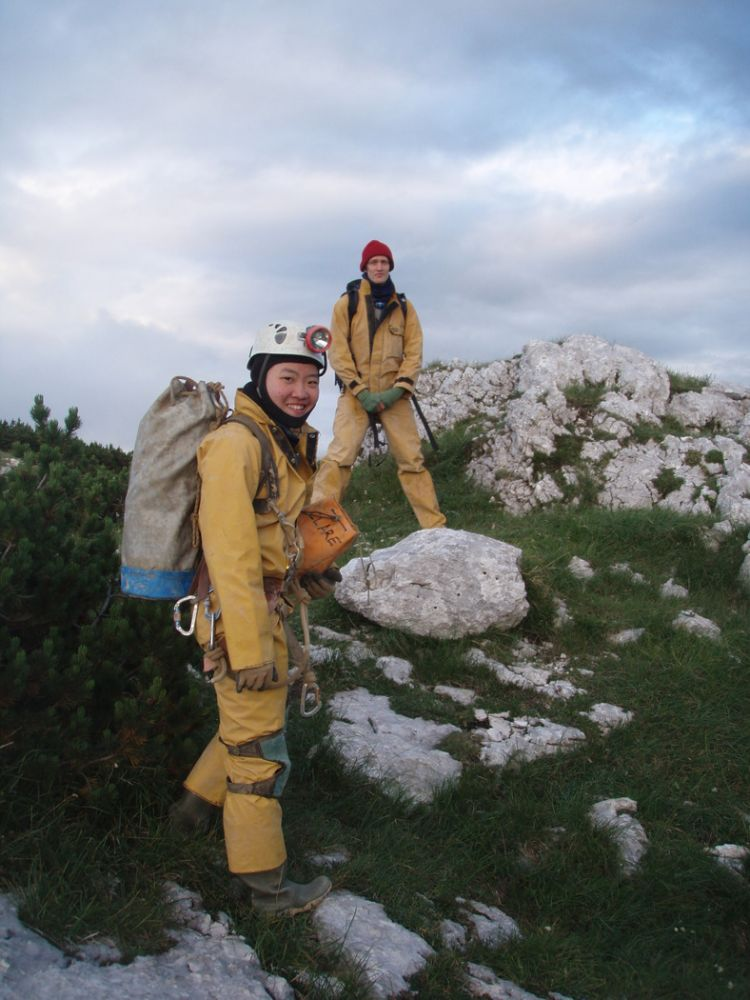
\includegraphics[width=\linewidth]{2011/alex_pitcher_award/2011-07-24-19.18.19-Jan Evetts-Olympus Compact-P7240049-Clare and Jarv off on first Camping Push--orig_1050p.jpg}} 
 \caption{After a spate of bad weather, Clare Tan and Jarvist Frost head off for a camping and pushing trip. \pic{Jan Evetts}}
 \label{clare jarv push}
\end{marginfigure}


The sunlight that greeted me at the entrance was blinding and I felt
overjoyed to feel the cold breeze of the plateau blow on my face and to
smell the sweetness of the air once again. I had spent roughly 72 hours
underground and descended to a depth of roughly 700 m but suddenly all
the low points of the journey faded and away and I was filled with the
euphoria of being above ground again. I couldn't wait to descend once
again.

Arriving at the \passage{Bivi}, everyone was huddled together seemingly battered
by the recent weather conditions and morale seemed quite low. Some of the
Slovenians had begun to arrive though, and it was especially great to
meet Izi again who I had been down \passage{Swildon's Hole} with earlier in the
year.


\begin{pagefigure}
\checkoddpage \ifoddpage \forcerectofloat \else \forceversofloat \fi
   \centering
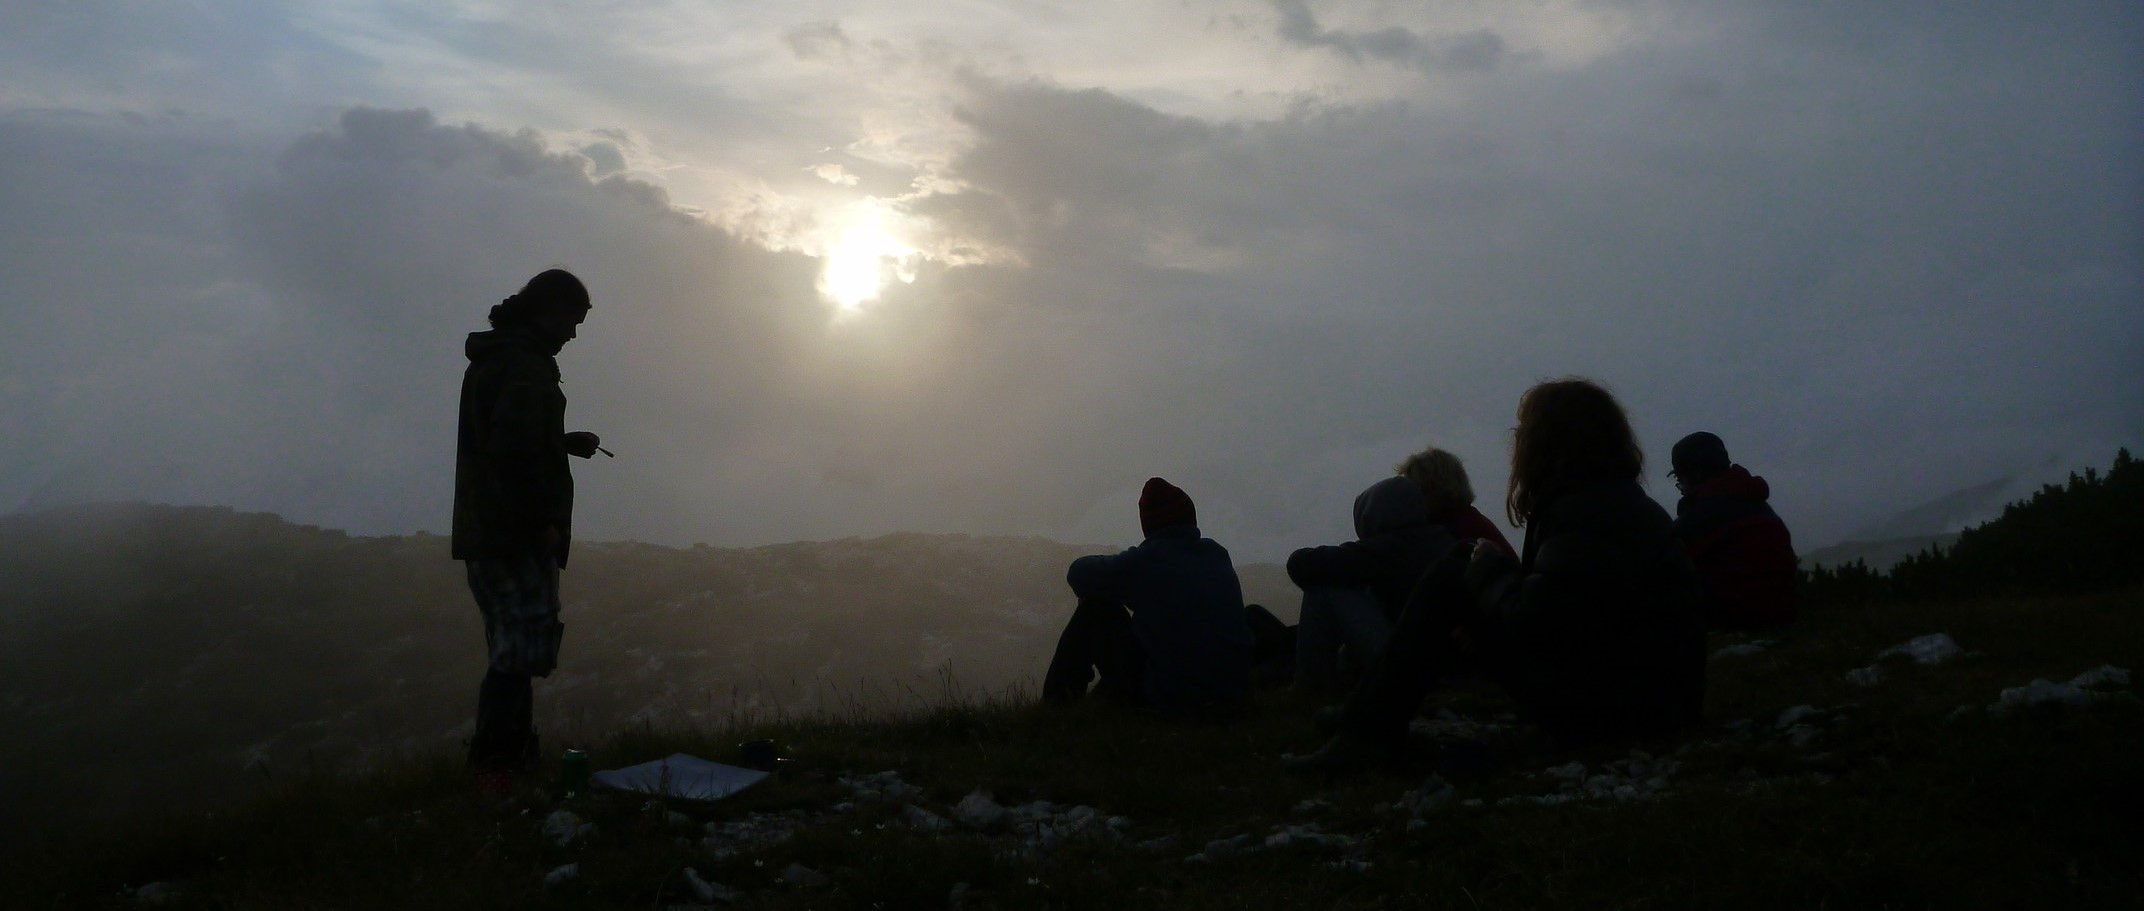
\includegraphics[width = \textwidth]{2011/alex_pitcher_award/2011-07-30-18.57.51-Grega-Panasonc DMC-FT2-019--orig.jpg}
\caption{A cloudy sunset, sometimes called "clagset", at sunset spot. \pic{Grega Maffi}} \label{cloudy sunset}
\end{pagefigure}


\subsection{A trip into SysMig}

In addition to \passage{Gardener's World} the other large cave on the plateau is
\passage{Sistem Migovec}, the cave that had originally the primary focus of the
expedition. One of the classic trips within \passage{Sistem Mig} was to bounce
down to an area known as \passage{Bikini Carwash}, a trip that takes in many great
traverses and serves to highlight the striking difference between the
two caves. After exiting \passage{Gardeners' World} Tetley agreed to take myself
and a couple of other cavers on this trip. Despite working in a group of
4 cavers feeling quite odd to begin with, the trip was relaxed and it
was inspiring to see what the generation of cavers before me had pushed,
especially the traverses above blackness. The trip ended in colossal
horizontal section of cave that was magnificent. I can't begin to
imagine how the cavers must have felt upon first discovering it,
especially after the relief of passing the tricky traverses that lay
before it.

\tweet{6:52PM Jul 23, 2011}{Last nec. carries complete, weather continues to be dire,lightning strikes on plateau etc.All rather tired with small team.Cave storms on.}

The journey out was again relaxed and gave me another opportunity to
work on my SRT technique. One hiccup occurred at the final pitch head,
however, when I decided to dive head first through a fairly small hole
with my cowstails clipped in to the rope. Finding myself stuck\sidenote{Getting briefly stuck is a common minor mishap at the entrance of \passage{M16}!}, I
decided to roll over so that I could dislodge myself. In doing so I
managed to wrap my leg quite firmly in my cowstails. In such a moment it
was quite difficult to remove from my thoughts ``PANIC, YOU'RE GOING TO
LOSE YOUR LEG'' despite how foolish it may seem now. Nevertheless,
untangling myself wasn't too much of a problem and I left the cave with
my leg intact.

\subsection{A break in Tolmin}

The next day I was slow to wake up and make my way to the \passage{Bivi}. Two
weeks into the expedition I had convinced myself that I would head down
to \passage[town]{Tolmin} for a couple days of rest before returning to underground
camp. Tetley had been due to head back underground that day with another
caver named Dave but Dave hadn't been feeling very well and had opted to
pull out of going underground. Tetley offered me Dave's place but I had
no problem with declining. I made plans to go underground with Dave
following a weekend in \passage[town]{Tolmin} and promptly headed to \passage[town]{Ravne}. From \passage[town]{Ravne},
I took a bike down the twists and turns to \passage[town]{Tolmin} before arriving in the
town. Now, when you live on top of a mountain with a group of cavers,
not washing for a couple of weeks seems perfectly viable. As you become
dirtier and smellier it's difficult to notice it as you only seem to
compare yourself with everyone around you. Considering that they haven't
washed either you seem perfectly at ease with your cleanliness. Upon
entering \passage[town]{Tolmin} by myself however, it became apparent to me that I
wasn't exactly clean as passing onlookers stared at me with mud still
caked on my face since my previous trip underground. I arrived at
\passage[town]{Tetley's flat}, where we stayed in \passage[town]{Tolmin}, and treated myself to one of
the best showers I have ever had, watching the water draining from the
shower turn a dark shade of brown with every shake of my hair.

Just as I was beginning to become tired of how quiet the flat was I saw
a pair of figures striding across the front lawn to \passage[town]{Tetley's flat}. Not
recognising either of them I went to greet them. One of them turned out
to be the much spoken about Fratnik, the senior caver of the JSPDT and
another man named Hugh who had been on a few of the earlier expeditions.
Hugh had been close to Slovenia undertaking a pottery course and had
decided to stop by. He also happened to have an inflatable raft with him
and, after a few pints and some ice cream we decided to raft down the
easier sections of the stunning river that is the \passage[river]{Soča}. The next day we
waited to see if a couple of other cavers who we were expecting to come
down the mountain would want to come rafting too but by lunchtime it
seemed that they wouldn't be in \passage[town]{Tolmin} any time soon. We promptly drove
further up the \passage[river]{Soča} and, in the midst of torrential rain, took to the
river.

\begin{marginfigure}
\checkoddpage \ifoddpage \forcerectofloat \else \forceversofloat \fi
\centering
 \frame{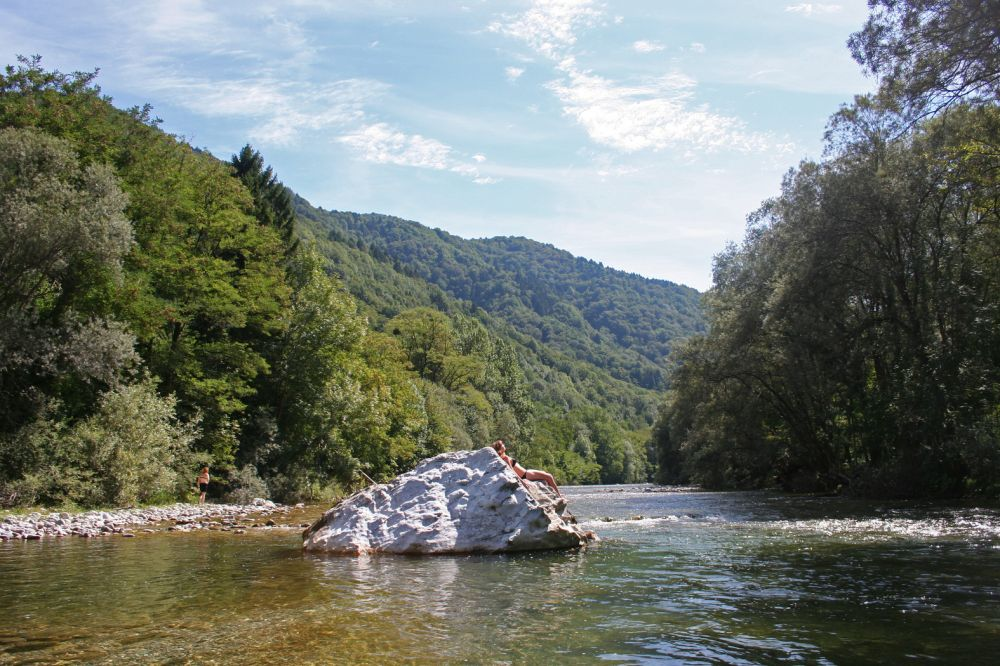
\includegraphics[width=\linewidth]{2011/alex_pitcher_award/2011-08-13-09.49.28-Jana Carga-Canon 350D--orig_1050p.jpg}} 
 \caption{The sparkling waters of the river \passage[river]{Soča}. \pic{Jana Carga}}
 \label{kate soca}
\end{marginfigure}

The journey was majestic as thunder clashed around us and rain piled
into the deep turquoise river. As the rain began to let off, a thick
mist rose from the river only heightening the sense that we were in a
truly beautiful country. Despite kayaking down one of the quietest
sections of the river we still came across a few rapids which, in our
poorly balanced inflatable raft, posed the threat of us being flung into
the freezing waters of the \passage[river]{Soča}. Thankfully, we avoided the water
although the act of Hugh abandoning me to stand on a precarious rock as
I floated down the rapids solo almost sunk our raft.

We returned to \passage[town]{Tolmin} elated by our journey to find one of the cavers we
were expecting, Jan. So that I could avoid the bike up the twists and
turns to \passage[town]{Ravne}, Jan gave me a lift up so that I could spend the night
there and set off early. We were greeted by the once again hospitable
family at \passage[town]{Ravne} who served us some fruit tea and cake before Jan and
Hugh returned to \passage[town]{Tolmin} and I retired to the van to spend a night in
relative comfort.


\tweet{7:22PM Aug 2, 2011}{Just in case you thought we were suffering too much,earlier rain and recent sun ripened raspberries@1500 \& blueberries@1850 to perfection!} 

I was awoken by the sound of Hugh's voice joined by someone who sounded
familiar. One of the caving freshers, Ari, had finally arrived in
Slovenia to join us on top of the mountain. We set off with our bags
loaded, the company providing a very welcome change from the now
repetitive carries up the mountain. Up top, everyone seemed to be in
much better spirits as three sections of the mountain had begun to yield
new cave. The \passage{Red Baron} had lead to an extensive horizontal
section of passage that ended in a pitch soon to be named `\passage{Stuck
in Paradise}' due to its extremely muddy nature. The other extensions
below \passage{Cheetah} that had lead to a group of wet pitches ending in
\passage{Serpentine} the year before were now being pushed down some more
pitches that I believe were called `\passage{It Will Rain}' and, finally,
the deepest section of the cave had now been pushed to an area known as
\passage{Daydreamers} adding the instant gratification of increasing the
depth of the cave. The hard work of the various cavers on the mountain
was finally paying off.

\name{Jonathon Hardman}
